\documentclass[a4paper]{scrreprt}

\usepackage[ngerman]{babel}
\usepackage[utf8]{inputenc}
\usepackage[T1]{fontenc}
\usepackage{ae}
\usepackage[bookmarks, bookmarksnumbered]{hyperref}
\usepackage{tabularx}
\usepackage{graphicx}
\usepackage{csquotes}
\usepackage{verbatim}
\usepackage{float}
\usepackage[nonumberlist, toc, section]{glossaries}
\usepackage[german]{fancyref}

\setcounter{secnumdepth}{4}

\begin{document}

\title{Implementierungsdokument CS:Select}
\author{Luca Springer, Alexander Linder, Julian Dinh, Nicholas Bieker,\\ Bendix Sonnenberg}
\maketitle

\tableofcontents


\chapter{Einleitung}

In diesem Dokument beschäftigen wir uns mit der Implementierungsphase unseres Projekts CS:Select. Dabei befassen wir uns insbesondere damit, welche Kriterien aus unserem Pflichtenheft wir umgesetzt haben und welche Änderungen sich zu unserem Entwurf ergeben haben. Da das Front-End im Entwurfsdokument nur sehr oberflächlich behandelt wurde, gehen wir nun nochmal genauer darauf ein, wie dieses gestaltet wurde. Außerdem stellen wir dar, wie die Implementierung zeitlich abgelaufen ist und welche Frameworks und Bibliotheken wir dabei benutzt haben. Schlussendlich gibt es einen einen Überblick über die bereits vorhandenen Unit-Tests.

\hspace{1cm}

Genereller Aufbau


\chapter{Implementierte Kriterien}

\section{Muss-Kriterien}
Alle Muss-Kriterien aus dem Pflichtenheft wurden bei der Implementierung berücksichtigt und alle zugehörigen Funktionellen Anforderungen sind implementiert.


\section{Kann-Kriterien}
Die folgenden Kann-Kriterien sind inklusive aller zugehörigen Funktionellen Anforderungen implementiert:
\begin{itemize}
\item Erweiterte Nutzerverwaltung (E-Mail-Adresse und Passwort ändern sowie Passwort zurücksetzen)
\item Zusätzliche Funktionen für den Organisator in der Übersichts-GUI (Spiele vorzeitig beenden und beendete Spiele aus der Übersicht löschen)
\item Speichern und Laden von Spieleinstellungen bei der Spielerstellung
\item Zusätzliche Optionen für den Spieler im Spiel (Runde überspringen, Merkmal als unwichtig markieren)
\item Gamification-Elemente Leaderboard, Achievements, Daily Challenges und Streaks
\item Bedienungshilfen %???
\item Internationalisierung (Sprache im Browser ändern, englisches Sprachpaket)
\end{itemize}

\hspace{1cm}

Weitere Kriterien sind teilweise implementiert, also sind manche zugehörige Funktionale Anforderungen implementiert, andere dagegen nicht:

\subsection{Zusätzliche Funktionen zur Verwaltung des Spiel-Servers}
Zusätzliche Funktionen zur Verwaltung des Spiel-Servers: Dadurch, dass alle Daten in unserer Datenbank gespeichert werden und nicht im Arbeitsspeicher gehalten werden, wird der Zustand des Spiel-Servers auch bei einem Neustart erhalten. Spiele und Organisatoren können direkt aus der Datenbank gelöscht werden. Die Kommunikation eines Administrators mit dem System über eine Kommandozeile ist dagegen nicht möglich und es gibt auch keinen Dialog beim Aufsetzen des Servers, da dafür die Config-Datei genug sein sollte.  

\subsection{Verbesserung der Merkmalsbereitstellung für ein Spiel}
Solange das möglich ist, wird das Anzeigen von gleichen Merkmalskombinationen in einem Spiel vom System verhindert. Bis auf diese Einschränkung erfolgt das Erzeugen der angezeigten Merkmalskombination jedoch zufällig.


\subsection{Unterstützung von mehreren Plattformen}
%???


\hspace{1cm}

Das letzte Kann-Kriterium, weitere Spielmodi, wurde dagegen aus Zeitgründen und aufgrund von einem Mangel an sinnvollen Ideen nicht umgesetzt.
\chapter{Änderungen zum Entwurf}

\section{API}

\section{User}

\section{Database}
\begin{itemize}
    \item Neue Param-Klassen zum parametrisierten Aufruf von Mysql-Prepared-Statements
    \item registerPlayer/Organiser Methoden zu createPlayer/Organiser umbenannt und den Registrierungsprozess ausgelagert
    \item FeatureSet Informationen werden nicht mehr in die DB geschrieben sondern verbleiben in der erhaltenen .json Datei auf der Platte
\end{itemize}

\section{GameCreation}

\section{Game}
\begin{itemize}
	\item Datentyp für Zeitpunkte ist LocalDateTime
	\item Features werden in FeatureSet als Set gespeichert, dementsprechend gibt die Methode getFeatures auch ein Set statt einer Collection zurück
	\item Methode getFinished von Game heißt nun isTerminated, da sie kein Getter ist sondern die Terminierung überprüft
	\item Methode getRounds von Game gibt Collection statt Liste zurück, da die Reihenfolge hier nicht relevant ist
	\item Entsprechend dem Vorgehen bei den Usern wird auch beim Game über die Datenbank sichergestellt, dass evtl. verschiedene Objekte zum gleichen Spiel synchronisiert sind, deshalb sind die Attribute invitedPlayersEmails und numberOfRounds sowie die Assoziationen zum Spieler und zur Runde über die Datenbank realisiert 
	\item Klasse Termination hat Setter-Methode für das zugehörige Spiel
	\item Die Rundennummer ist nicht relevant und wurde somit nicht implementiert, deswegen ändern sich auch die Signaturen der entsprechenden Fabrikmethoden der Spielmodi
	\item Klasse GamemodeComposite hat getGamemode Methode
	\item Die Methoden skip und selectFeatures der Klasse Round benötigen keine Feature-Objekte, sondern nur deren ID, deshalb wurde die Methodensignatur entsprechend geändert, genauso auch die Methode acceptInvite der Klasse Game mit der \newline PlayerID statt einem Objekt
	\item Bei der provideFeatures-Methode ist die Reihenfolge der erzeugten Features relevant, deshalb ist hier nun der Rückgabetyp eine Liste statt einer Collection
	\item Runden haben eine setGame Methode
	\item Die Boolean-Rückgabewerte der Methoden invitePlayers, acceptInvite und declineInvite waren unnötig und wurden rausgenommen
\end{itemize}
\section{Gamification}

\section{Sonstiges}
\begin{itemize}
    \item Configuration, MLServer und DatabaseAdapter jetzt Interfaces zur Injection mit Google Guice
    \item DefaultConfiguration umbenannt zu ApacheCommonsConfiguration nach der genutzten Bibliothek
\end{itemize}

\chapter{Front-End}

\chapter{Frameworks und Bibliotheken}

\chapter{Zeitlicher Ablauf}

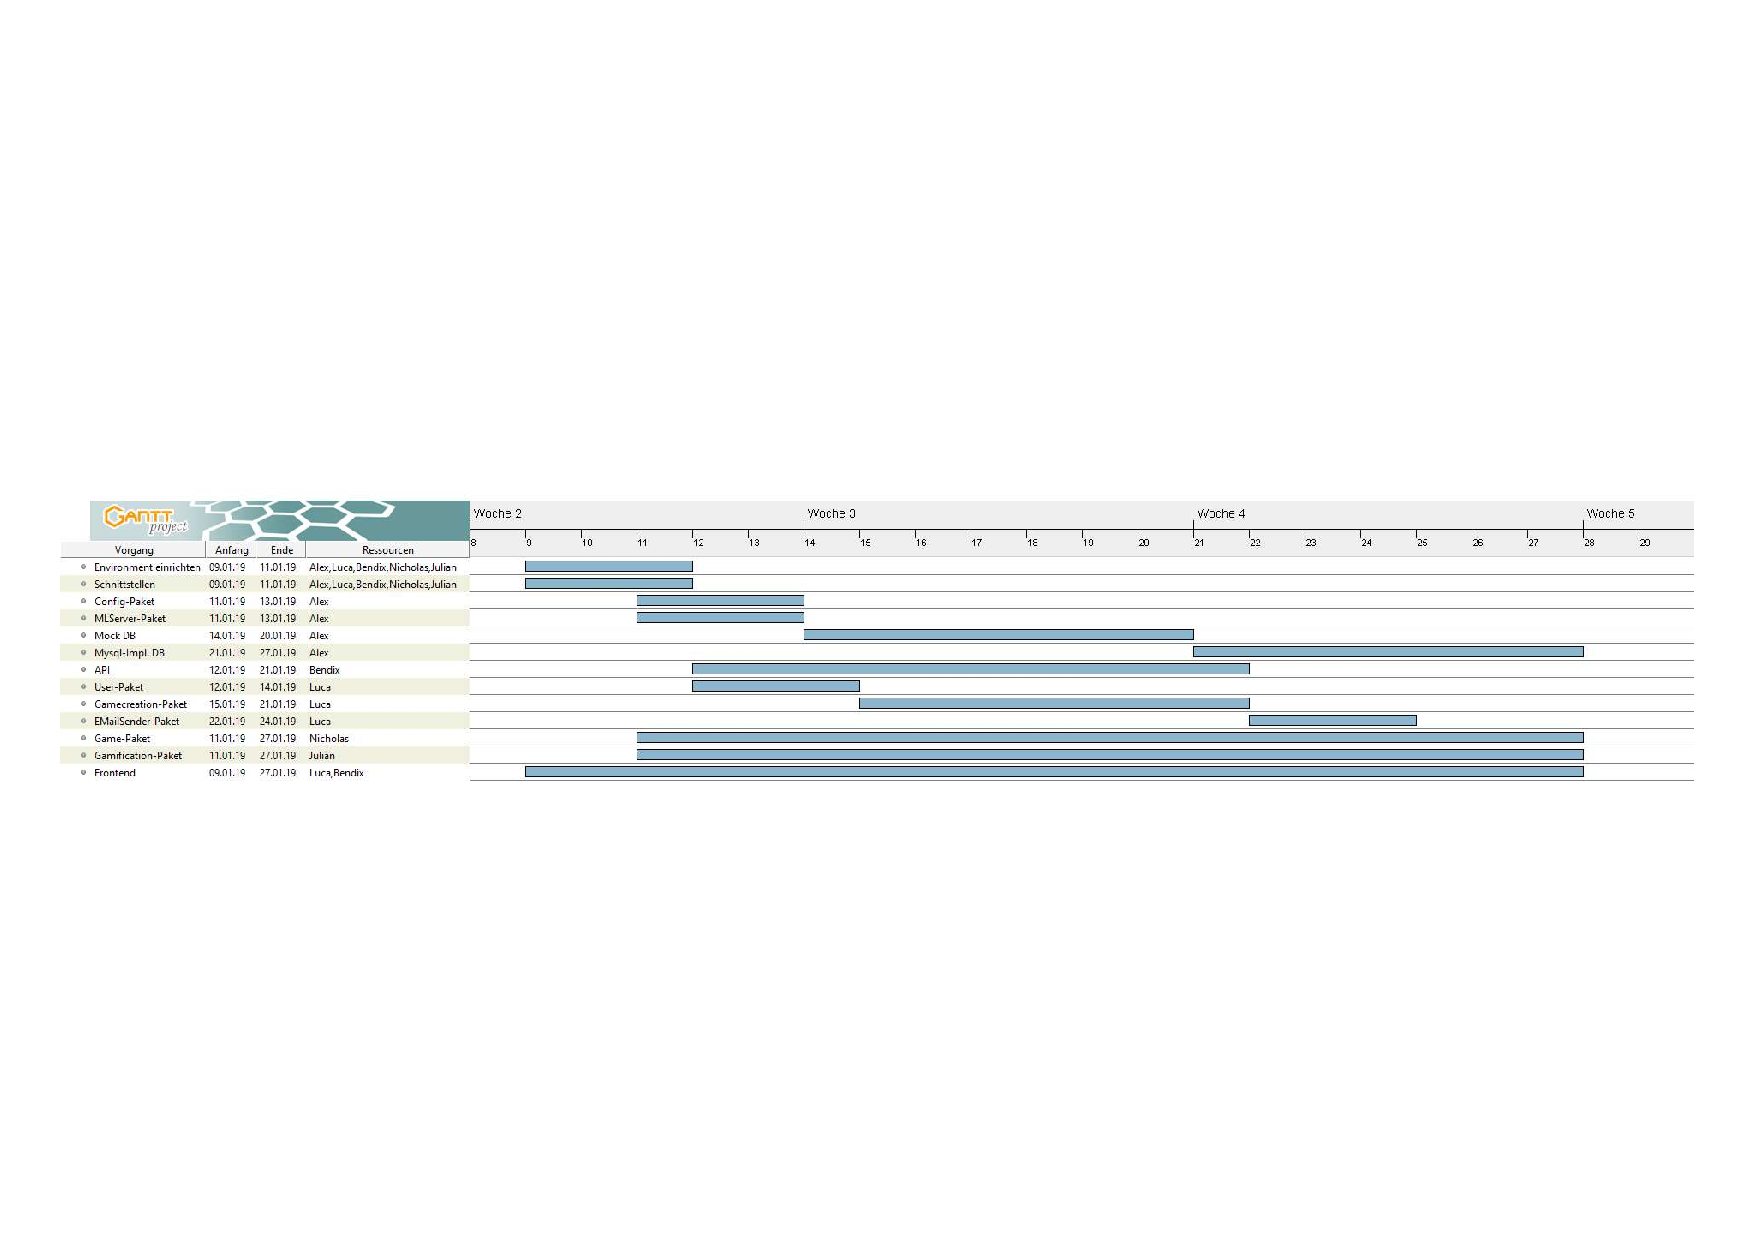
\includegraphics[width=\linewidth]{img/gantt.pdf}

\chapter{Unit-Tests}






\end{document}